\section{Results}

\subsection{Phase 1: LLM Labeling}

\begin{table}[!ht]
\centering
\caption{\textbf{Labeler Statistics}}
\label{tab:labeler-results}
\begin{tabular}{lllccc}
\toprule
 &  &  &  \textbf{LPP} & \textbf{Cost} & \textbf{M.-F1} \\
\textbf{Model} & \textbf{Context} & \textbf{Shot} & ($\mu\pm\sigma$) & (\$) & (\%) \\
\midrule
\multirow[c]{6}{*}{
    \rotatebox[origin=c]{90}{GPT-3.5}
    } & \multirow[c]{2}{*}{\texttt{context1}} & 0-shot & 0.39 ± 0.61 & \textbf{0.36} & 15.96 \\
 &  & 1-shot & 0.91 ± 0.95 & 0.48 & 23.26 \\
 & \multirow[c]{2}{*}{\texttt{context2}} & 0-shot & 1.39 ± 0.98 & 0.42 & 37.59 \\
 &  & 1-shot & 1.68 ± 1.15 & 0.63 & 38.69 \\
 & \multirow[c]{2}{*}{\texttt{context3}} & 0-shot & 1.57 ± 1.08 & 0.57 & 37.24 \\
 &  & 1-shot & 1.85 ± 1.24 & 0.80 & 37.70 \\
\midrule
\multirow[c]{6}{*}{
    \rotatebox[origin=c]{90}{GPT-4}
    } & \multirow[c]{2}{*}{\texttt{context1}} & 0-shot & 1.50 ± 0.93 & 4.68 & 35.55 \\
 &  & 1-shot & 1.83 ± 1.36 & 5.75 & 36.10 \\
 & \multirow[c]{2}{*}{\texttt{context2}} & 0-shot & 2.16 ± 1.03 & 5.26 & 45.39 \\
 &  & 1-shot & 2.49 ± 1.28 & 7.25 & 45.93 \\
 & \multirow[c]{2}{*}{\texttt{context3}} & 0-shot & 2.30 ± 1.11 & 6.68 & 44.10 \\
 &  & 1-shot & 2.80 ± 1.30 & 8.99 & \textbf{46.12} \\
\bottomrule
\end{tabular}
\end{table}


Table~\ref{tab:labeler-results} presents important statistics of the re-labelling of the original crowdsourced corpus of websites using the LLM labelers introduced in Section \textit{Link to Methods}.

% General Results: Consistency, Cost, Quality
\textbf{Results.} Our findings demonstrate that LLM labelers can provide \textit{consistent}, \textit{cost-effective}, and \textit{high-quality} annotations for the complex task of multi-lingual, multi-label website topic classification. Remarkably, not a single incorrect output was produced, underscoring the reliability and consistency of LLM-generated annotations.

In terms of cost, the original paper~\cite{homepage2vec} cites an annotation expense of approximately \$143 per 1000 pages. Our approach, utilising GPT-3.5 and GPT-4 labelers, drastically reduces this cost to an average of \$0.60 and \$6.30, respectively, achieving a reduction by factors of 238x and 23x.

Performance-wise, GPT-4 peaks at a 46\% macro F1 score using context 2 and 1-shot, outperforming the baseline of the pre-trained model. The improvements suggest that we can expect to improve the performance of the pre-trained model by fine-tuning it with the LLM labels if we can distil the knowledge from the LLMs into the pre-trained model - the goal of the second phase of our study.

% GPT labeler parameter grid
\textbf{Labeler Parameter Grid.} Figure~\ref{fig:labelers-grid} visualises the effect of the labeler parameters on the macro F1 score. As expected, we find that the quality of the labels increases with the amount of context provided and the quality of the model used. Interestingly, the added features in context 3 (links and texts) do not increase the annotation quality, which is not surprising given the marginal improvements the original paper reported and the danger of confusing LLMs with prompts that are too complex as found in \textit{CITE}.

\begin{figure}[!h]
    \centering
    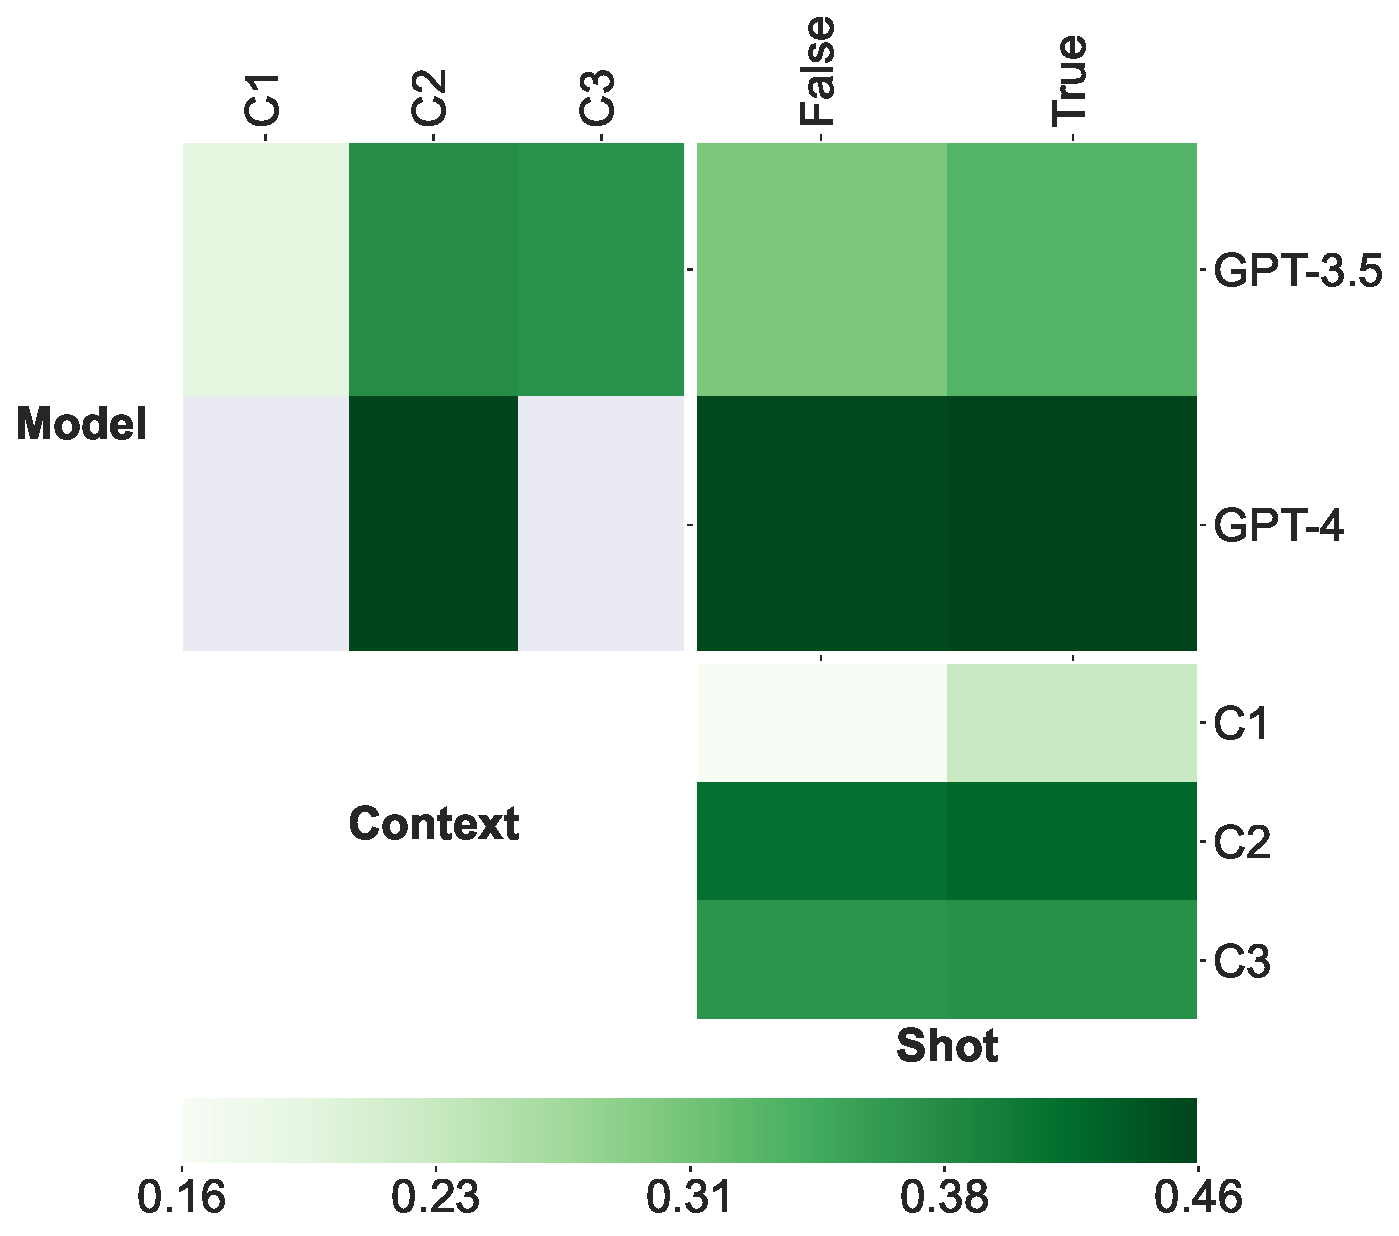
\includegraphics[width=.8\columnwidth]{./figures/labelers-grid.pdf}
    \caption{\textbf{Labeler Parameter Grid.} The Figure displays the mean macro F1 score for all unique parameter combinations of the LLM labelers.}
    \label{fig:labelers-grid}
\end{figure}

% Cost-quality trade-off
\textbf{Cost-Quality Trade-Off.} Our analysis reveals a direct correlation between label quality and cost, attributable to the use of longer prompts or more sophisticated models. The optimal compromise is achieved with a GPT-3.5 annotator utilizing context 2 and a few-shot example. This configuration ensures a robust label quality at 39\% (only a 15\% decrease) while cutting the cost per 1000 pages from \$7.25 to \$0.63 (a 91\% decrease). This GPT-3.5 annotator will be employed in the second phase of our study.

\subsection{Phase 2: Knowledge Distillation}

In the second phase of our study, we aim to improve the performance of the pre-trained model by fine-tuning it on a subset of the Curlie dataset, re-annotated with the best labeler from Phase 1 to represent the true label distribution more accurately. 

% 1. Step: Creating the dataset
We use GPT-3.5 using \texttt{context2} and \texttt{1-shot}.

with the LLM labels. We hypothesise that the LLMs can provide a more accurate and consistent supervision signal than the crowdsourced labels, which are prone to noise and inconsistencies. We also expect that the LLMs can provide a more diverse supervision signal, as they are trained on a much larger corpus of websites than the crowdsourced labels.

% Results:
 
% 2. Step: Fine-tuning
% - Show LPPs predicted
% - Visualise class-wise precision, recall and F1 (all macro)

% Something along the  lines:
% - We show that we can improve the Macro F1 score overall performance from 0.38 to 0.42, consistency outperforming the pre-trained model
% - Higher LPPs assigned

% Calculations
% Human annotator cost: 327 USD % Pages annotated: 761 * 3 = 2283
% Cost per 1k page: 1000 * 327 / 2283 = 143$

% GPT labler cost/1k pages:
% (0.36 + 0.48 + 0.42 + 0.63 + 0.57 + 0.80 + 5.26 + 7.25) / 8 = 2.6

% GPT-3.5 labler cost/1k pages:
% (0.36 + 0.48 + 0.42 + 0.63 + 0.57 + 0.80) / 6 = 0.6

% GPT-4 labler cost/1k pages:
% (5.26 + 7.25) / 2 = 6.3

% Cost reductions:
% GPT-3.5: 143 / 0.6 = 238x
% GPT-4: 143 / 6.3 = 22.7x